\chapter{The CMS experiment at the LHC}
\label{chap:detector}

\chapterquote{Traditional scientific method has always been, at the
very best, 20-20 hindsight. It's good for seeing where you've been.
It's good for testing the truth of what you think you know, but it
can't tell you where you ought to go.}%
{Robert M. Pirsig, Zen and the art of motorcycle maintenance}

The \LHC is one of the largest machines ever built. It exists within a
27~km tunnel $\sim 100$~m$)$ underground on the border of France and
Switzerland. Around the ring of the \LHC are built a series of
detectors that can record in a high level of detail the result of high
energy particle collisions produced by the collider. This chapter
will focus on the details and performance of \CMS, a multi-purpose
detector optimised to search for new, as yet undiscovered, particles.

\section{The LHC}
\label{sec:lhc}

The \LHC is a hadron collider designed to collide protons and lead
ions at centre of mass energies up to 14\tev, the highest ever achieved by such a
machine
\cite{Evans:2008zzb,CERN-2004-003-V-1,CERN-2004-003-V-2,CERN-2004-003-V-3}.
The proton-proton collisions are most utilised for direct searches for
new physics and therefore take up the vast majority of the \LHC's
running time. 

To bring protons up to the $6.5~\tev$ required in Run~2 of the \LHC
they are accelerated through a series of stages. Hydrogen atoms are
initially stripped of their electrons and accelerated to 50\mev by
\ac{LINAC2}. The energy is then increased to 1.4\gev by the \ac{PSB}
before being injected into the \ac{PS} which boosts the energy up to
26\gev. A final kick up to 450\gev is provided by the \ac{SPS}. This
chain of accelerators also collect the protons into bunches that are
either 25~ns (from Run~2 onwards) or 50~ns apart (during Run~1 and
early stages of Run~2). These bunches are then injected into the \LHC,
in which they are steered by around 1200 superconducting dipole
magnets while being accelerated up to $6.5\tev$ with \ac{RF} cavities.
Once the beam has reached the intended energy and is stable, protons
are collided at four different points on the ring, around which are
built the four major \LHC detectors, ALICE \cite{Aamodt:2008zz}, ATLAS
\cite{Aad:2008zzm}, LHCb \cite{Alves:2008zz} and \CMS
\cite{Chatrchyan:2008aa}.  A representation of this accelerator
complex and the location of the detectors can be seen in
Fig.~\ref{fig:lhc}.

\begin{figure}
  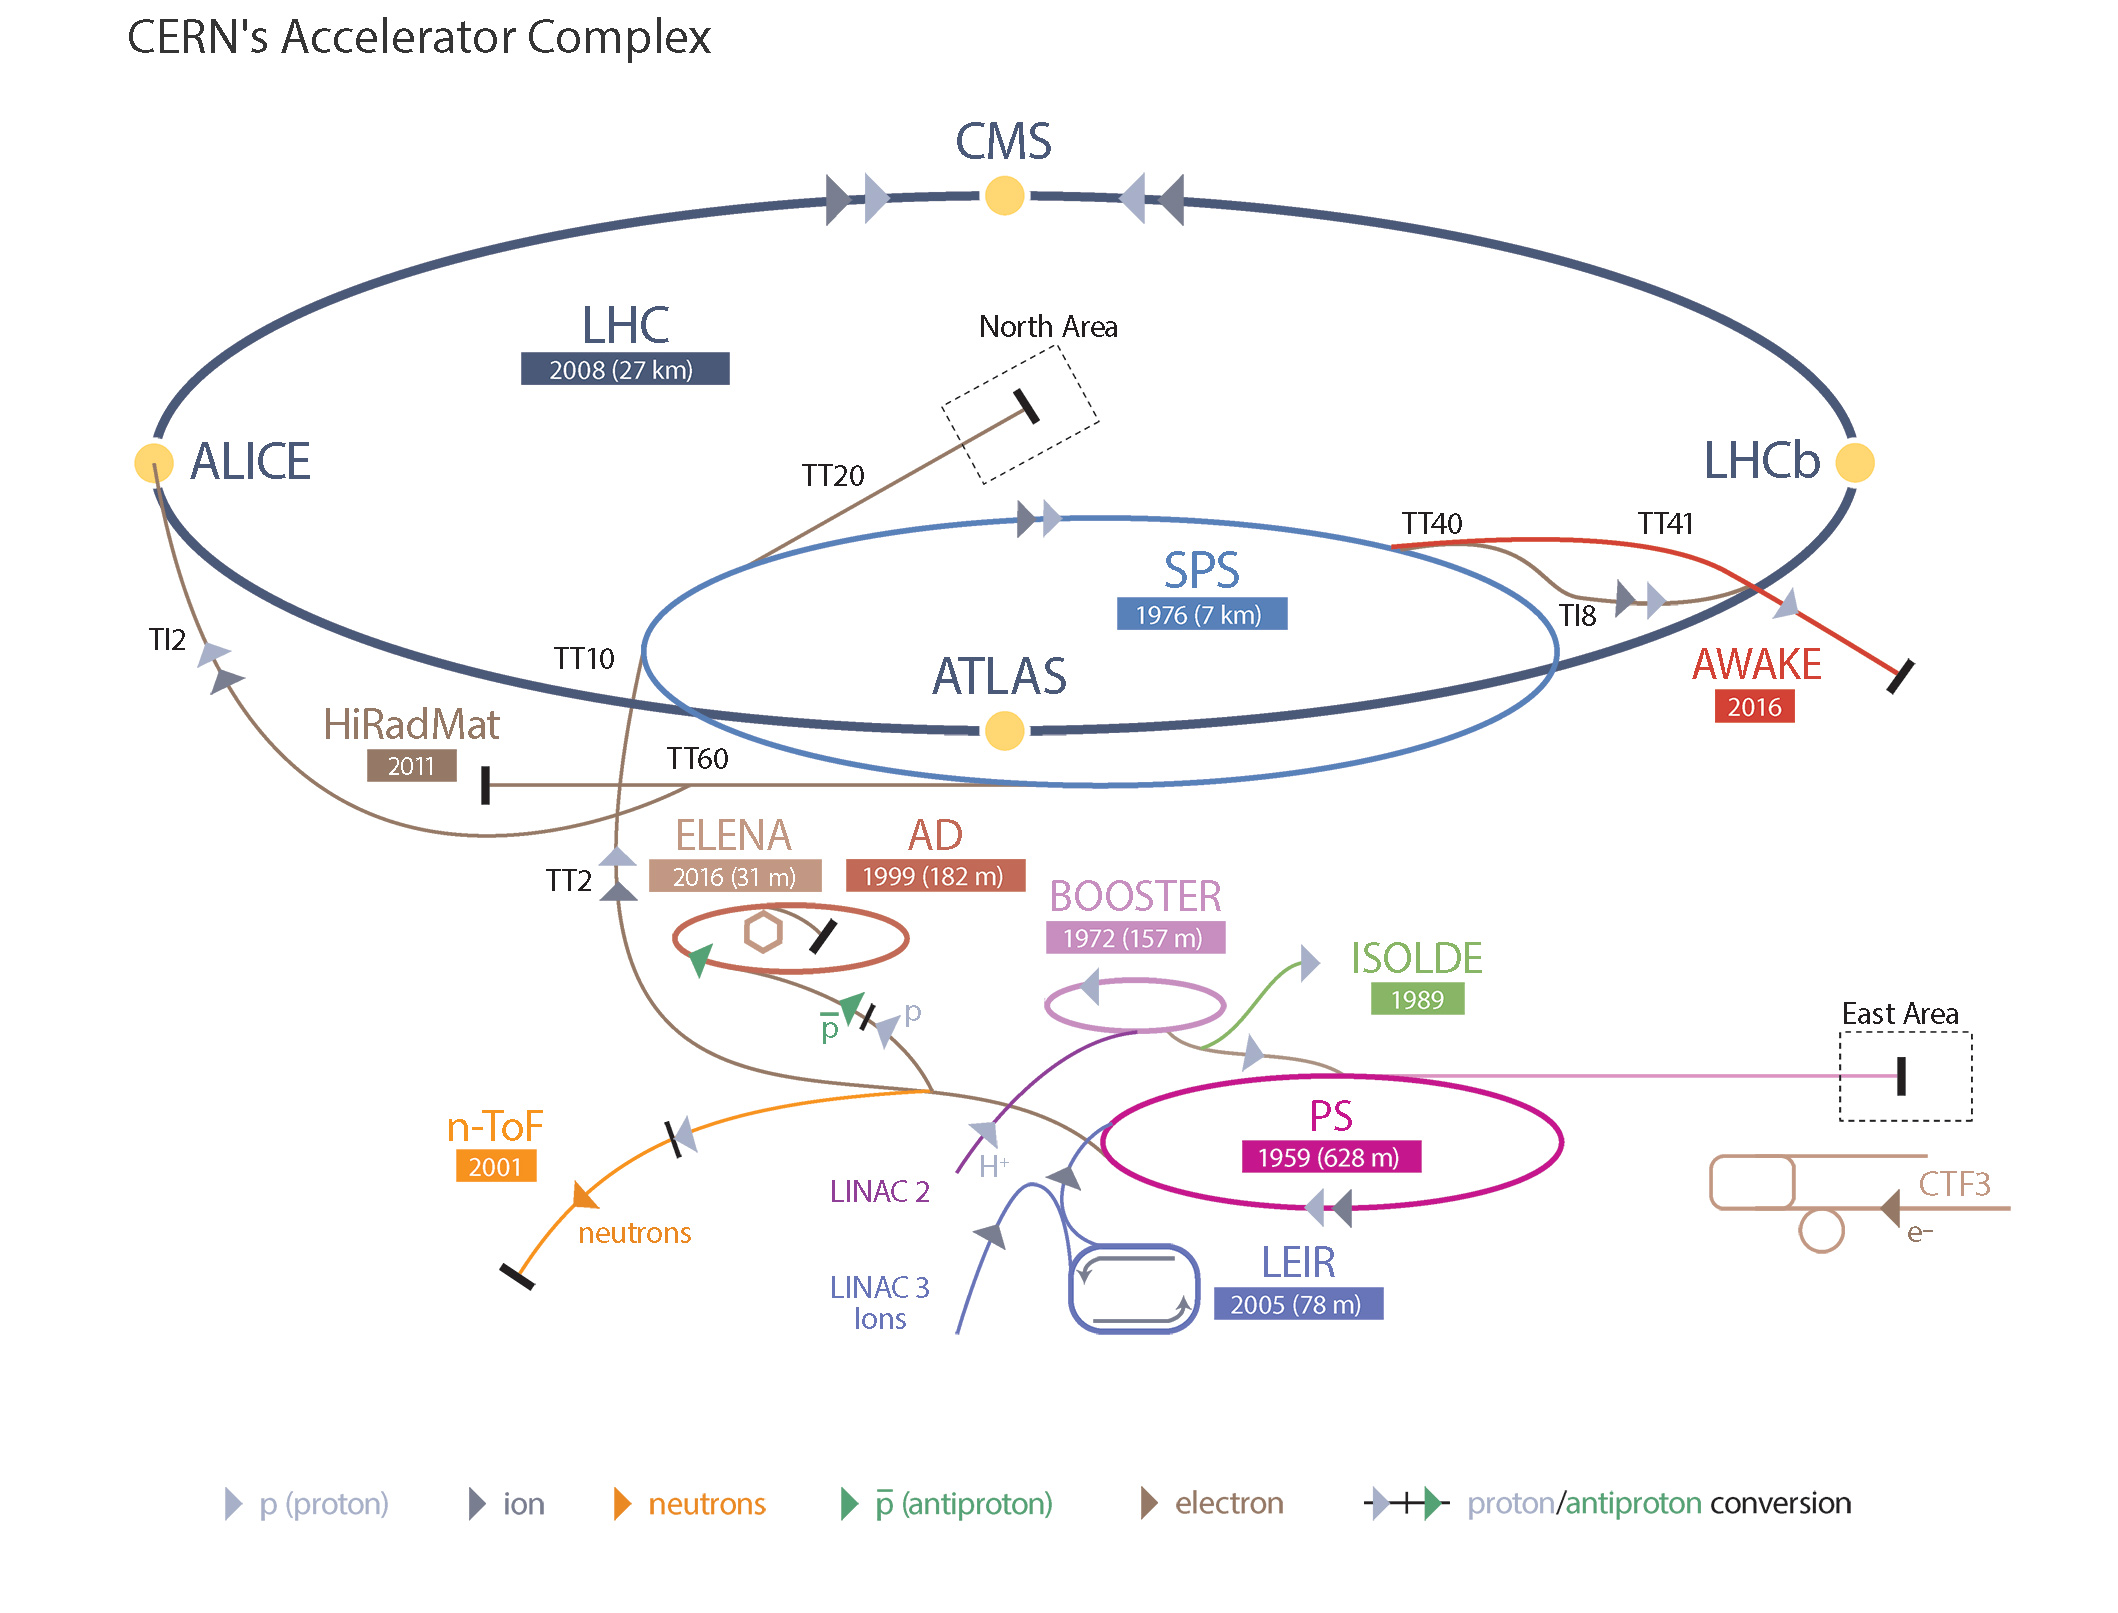
\includegraphics[width=\largefigwidth]{figs/LHC_default}
  \caption[]%
  {A representation of the CERN accelerator complex that help
  accelerate protons to record energies within the \LHC
  \cite{stfc:lhc}}%
  \label{fig:lhc}
\end{figure}

As well as attaining record breaking energies, the \LHC is designed to
collide hadrons at a very high luminosity, with a bunch collision rate
of up to $40~\mhz$ \cite{Evans:2008zzb}. This is necessitated by the
fact that the rate at which electroweak scale processes
occur in proton collisions is significantly lower than their
associated backgrounds, demonstrated in Fig.~\ref{fig:xsecs}.
The \LHC is therefore designed to run at an instantaneous
luminosity approaching $10^{34}$cm$^{-2}$s$^{-1}$ to maximise the occurence of
these rare processes. Along with the high collision rate, this
luminosity is achieved by squeezing the proton bunches to increase the
number of simultaneous collisions per bunch crossing, the extra
simultaneous collisions are known as \PU.  The \LHC has typically
operated with a \PU of $\sim10\mbox{-}20$, however to increase the
luminosity in the future this value will be increased up to a \PU of
O(100).
% , presenting a significant challenge for current and future 
% physics analyses at the \LHC.

\begin{figure}
  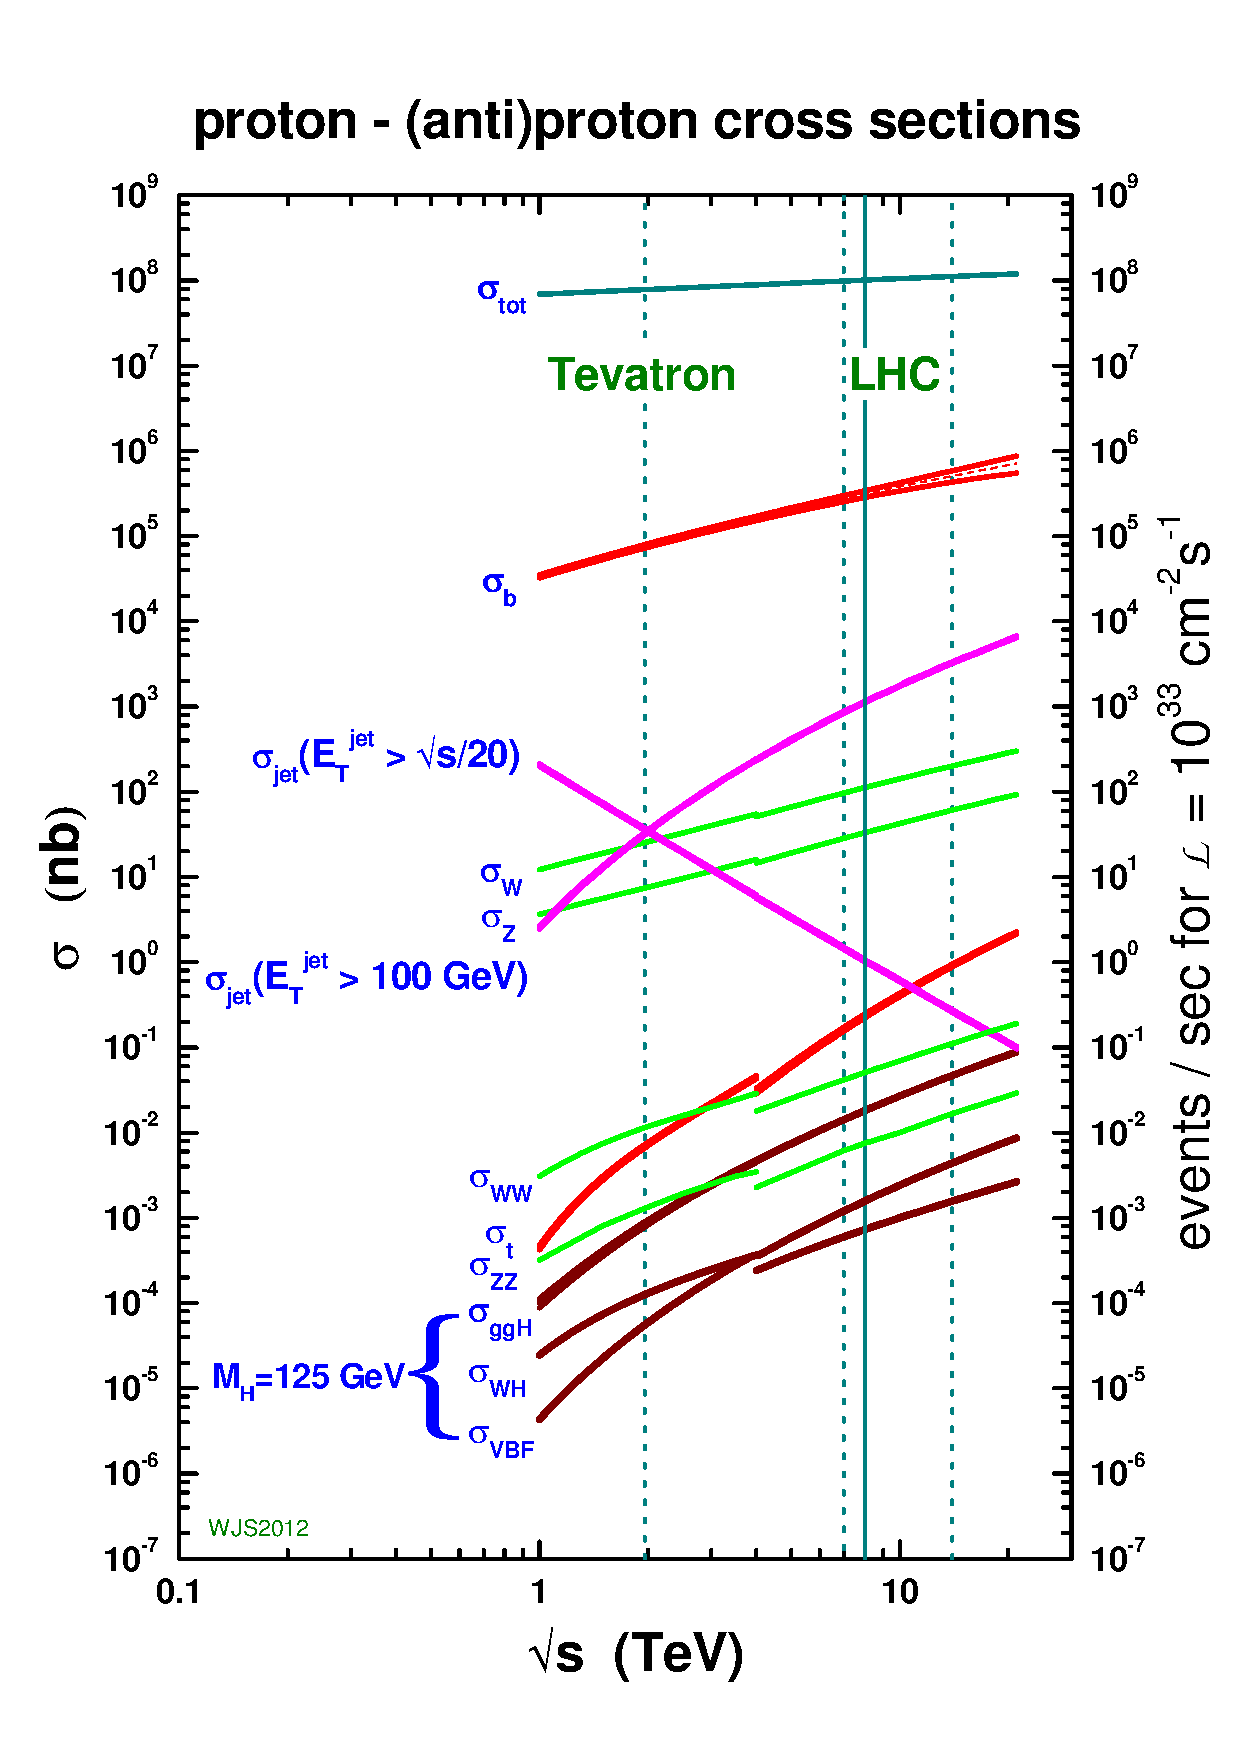
\includegraphics[width=\mediumfigwidth]{figs/crosssections2012_v5}
  \caption[]%
  { The cross sections for various standard model processes as a
  function of proton collider energy, demonstrating the importance of
  high luminosities when observing electroweak scale processes
  \cite{stirlingCrossSec1}.}%
  \label{fig:xsecs}
\end{figure}

During Run~1 of the \LHC, from 2010-2013, a total of $23.3~\ifb$ of
data were collected at centre of mass energies of $\sqrt{s}=7~\tev$ and
$8~\tev$. After this there was a period of shutdown in which the \LHC
and the detectors underwent a series of upgrades. Run~2 then began in
2015 with the collision of protons at $\sqrt{s}=13~\tev$. During 2015 a
total of $4.3~\ifb$ were collected at this energy. So far in 2016 the
\LHC has delivered $34.6~\ifb$, a record breaking number of collisions
at the highest ever recorded energies. 

\section{The CMS detector} \label{sec:cms}

The \CMS detector is one of two multipurpose detectors built around
proton beam collision points, the other being ATLAS. It is situated at
Point 5 on the \LHC, as visibile in Fig.~\ref{fig:lhc}. The key goals
of the \CMS detector at its conception were the discovery of the \SM
Higgs boson and searches for generic signatures of \BSM physics. In \CMS the
results of collisions are measured with a series of subdetectors,
built within and around a $3.8~$T superconducting solenoid. They are designed to
track, identify and record the energy of all non-neutrino \SM particles
\cite{Bayatian:2006zz}. With its comprehensive solid
angle coverage, \CMS is well suited to inferring the existence of
weakly interacting particles through the momentum imbalance of visible
particles. This is particularly relevant when searching for \BSM
physics.

\begin{figure}
\begin{center}
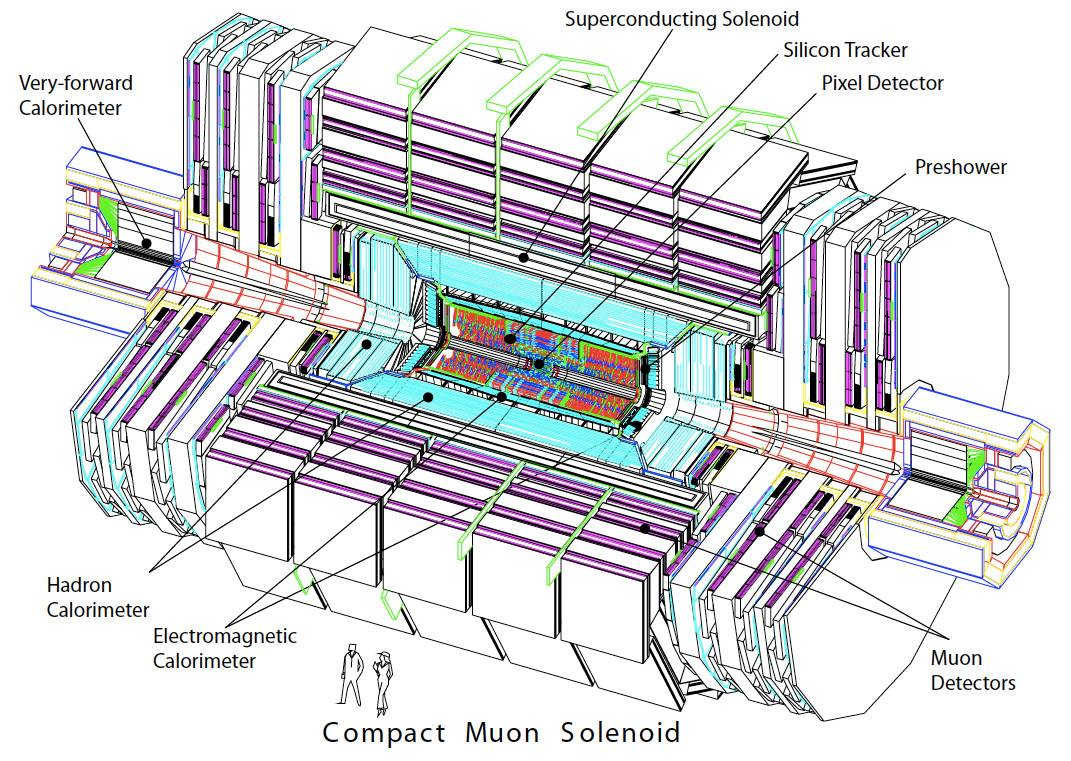
\includegraphics[width=0.8\linewidth]{figs/cms_detector} \end{center}
\caption{An internal view of the \CMS detector
highlighting the key detecting components \cite{Bayatian:2006zz}}
\label{fig:CMS} \end{figure}

A representative view of \CMS and its components can be seen in
Fig.~\ref{fig:CMS}. The detector is designed in a series of
cylindrical layers of subdetectors working out from the central point,
where the proton collisions occur. The first layer consists of the
silicon tracking system. This tracker is designed to allow the
reconstruction of the trajectory of charged particles produced in the
collision point as they move through the magnetic field. The degree to
which the path of these particles is bent allows for an accurate
determination of their momenta. The next layer beyond the silicon
tracker is the \ECAL, which is designed to absorb and measure the
energy of electrons and photons. Surrounding this is the \HCAL that
absorbs the remaining hadronic particles that have punched through the
\ECAL. Built around the tracker and calorimeters is the superconducting
solenoid. In the final layer are the muon chambers and iron return
yoke. The chambers are designed to detect the presence of muons that
will not be absorbed by the central components of the detector. The
data from all these subdetectors are read out by dedicated front end
electronic. They are then passed through the \CMS trigger system which
selects the most promising data to be kept and stored for ``offline''
processing. 

Measurements of physical quantities made by \CMS are typically
interpreted in a three dimensional coordinate system that originates
from the centre of the detector. The $x$-axis points south, to the
centre of the \LHC ring, the $y$-axis points vertically upwards and
the $z$-axis points along the direction of the \LHC beam pipe. It is
then helpful to define the azimuthal angle $\phi$ which is in the
$x$-$y$ plane and measured relative to the $x$-axis. Measurements of
momentum and energy in this plane are described as transverse and
known as \pt and \Et respectively. The polar angle $\theta$ is then
defined as relative to the $z$-axis. This angle is used to construct
the pseudorapidity, defined as $\eta=-ln(tan(\theta/2))$. Distances in
the $\eta$-$\phi$ plane is then given as $\Delta R =
\sqrt{\Delta\phi^2+\Delta\eta^2}$.

\subsection{The tracker} 

The \CMS inner tracking system is designed to accurately determine the
trajectories of charged particles produced in hadron collision events
\cite{Karimaki:368412}. In the presence of the strong magnetic field
provided by \CMS's solenoid, the curvature of these tracks can be used
to reconstruct momenta with a resolution between $1.5\%$ and $3\%$ for
$p_T\sim 100$~GeV charged particles. The tracker is also capable of
tracking \mbox{$p_T>1$~GeV} charged particles with an efficiency
greater than $99\%$ \cite{Bayatian:2006zz}. Along with this, the
spatial resolution of the tracker is such that the points of origin of
event decay products can be inferred within $10$~$\mu$m. Together,
this allows the performance of \CMS to extend up to very high levels
of \PU.% \cite{CMSTrackPerformance}.

The tracker is required to operate in a challenging, high radiation
environment. Additionally, in an ideal detector the particles produced
in collisions are solely absorbed by the calorimeters. The tracker
must therefore consist of as little material as possible. To achieve
the high level of precision and fast response time required given
these conditions, the tracker utilises silicon technology. As charged
particles pass through doped silicon an electron-hole pair is
produced. In the presence of an electric field this gives rise to a
pulse of electrical current in the previously resistive silicon. This
behaviour is utilised by the tracker in a series of silicon pixel and
strip detectors covering all angles in \phi and extending up to
$|\eta|<2.5$. The tracker's layout is visible in
Fig.~\ref{fig:tracker}. 

\begin{figure}
\begin{center}
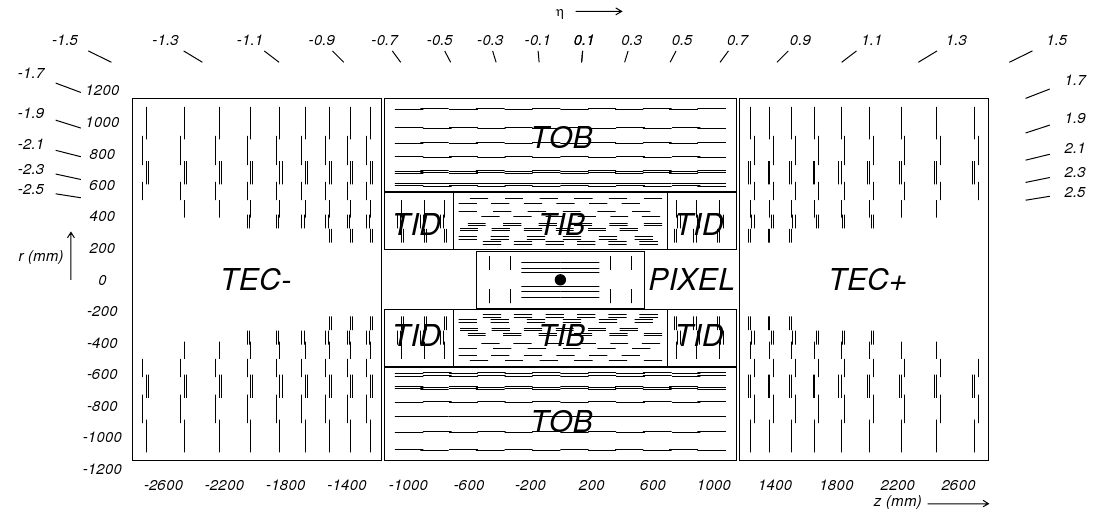
\includegraphics[width=0.8\linewidth]{figs/cmstracker} \end{center}
\caption{ A schematic of a cross section through the \CMS tracker.
Detector modules are represented by different lines \cite{Chatrchyan:2008aa}}
\label{fig:tracker} \end{figure}

The pixel detector is the high granularity component of the tracking
system that sits closest to the interaction point, covering the
pseudorapidity region $|\eta|<2.5$. It consists of three cylindrical
layers of hybrid pixel detector modules that are complemented by two
disks of pixel modules on each side. The pixel detector makes use of
66 million pixels covering an area of $\sim 1$~m$^2$ to give the
tracker its excellent spatial resolution of $15$-$20$~$\mu$m in both
the $r$-$\phi$ and $z$ direction. This resolution is essential for a
precise determination of the position of collision event vertices and
for the observation of vertices displaced from this origin that can be
used to identify particles such as hadrons containing $b$-quarks.

Surrounding the pixel detector is the silicon strip tracker that
covers the region up to $|\eta|<2.4$. It consists of three different
subsystems built from 9.6 million silicon strips that cover an area of
198~m$^2$. Each of these strips are 10-20~cm long and 80-180~$\mu$m
wide. Working out from the centre the subsystems are the
Tracker Inner Barrel and Disks (TIB/TID), the Tracker Outer Barrel
(TOB) and the Tracker End Caps (TEC). They are arranged in a geometry
that maintains a good degree of coverage across all angles and can be
seen in detail in Fig.~\ref{fig:tracker}. Along with the spatial
resolution provided by the pixel detector the silicon strip tracker
adds enough modules to reconstruct the trajectory of particles to the
required high level of precision.

\subsection{The electromagnetic calorimeter} 

The \ECAL is constructed from $\sim 75~848$ lead tungstate (PbWO$_4$)
scintillating crystals covering the region $|\eta|<3$ \cite{CMS:1997ema}. It is
designed to absorb electrons and photons and emit light proportional to the
energy deposited. This light is detected by custom photodiodes that
perform well in high magnetic fields. This is achieved in a way which
is fast, radiation resistant and with a high granularity. 

The \ECAL is divided into the \ac{EB} which covers the region
$|\eta|<1.479$ and the \ac{EE} which covers the region
$1.479<|\eta|<3.0$. Additionally, built just before the \ac{EE} in the
region $1.653<|\eta|<2.6$ is the Preshower. Unlike the other
components, which are predominantly PbWO$_4$ crystals, the Preshower is
a lead and silicon sampling calorimeter. Its main aim is to improve
the position resolution of particles in the forward direction and help
to distinguish collinear $\pi^0$ decays from high energy photons
\cite{Chatrchyan:2008aa}. This layout of the \ECAL can be seen in
Fig.~\ref{fig:ecal}.

\begin{figure}
\begin{center}
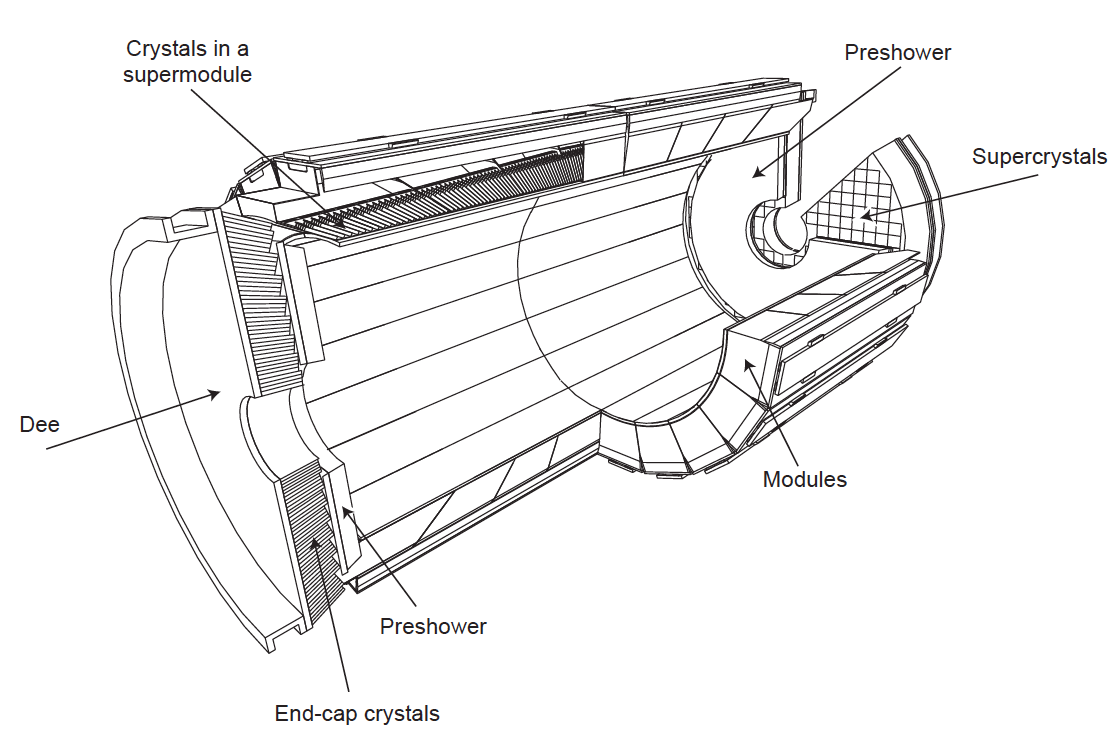
\includegraphics[width=0.8\linewidth]{figs/ecal_colorless} \end{center}
\caption{ A cutaway diagram of the \CMS \ECAL. All the key components,
including the barrel and endcap crystal layouts, are displayed
\cite{Chatrchyan:2008aa}}
\label{fig:ecal} \end{figure}

As high energy electrons or photons enter one of the \ECAL's crystals
they initiate an electromagnetic shower. This results in a cascade of
lower energy particles that undergo bremsstrahlung and pair
production.  These charged particles ionise atoms in the crystal which
then emit scintillation light as they de-excite. As the crystals are
transparent, this light can be measured by avalanche photodiodes and
vacuum phototriodes which convert it into an electronic current. The
magnitude of this current is then proportional to the energy deposited
in the crystal and can be used to accurately infer the total energy
deposited. Irradiation of the crystals decreases their transparency
over time. To counteract this a time dependent calibration is carried
out for each of the crystals with a laser of wavelength
$\lambda=440$~nm. 

Measurements in a test beam in the absence of a magnetic field have
measured the PbWO$_4$ crystals to have a resolution, $\sigma_E$, given
by the following formula \cite{1748-0221-2-04-P04004}:
\begin{equation} \label{eq:ecalres}
\left(\frac{\sigma_E}{E[\gev]}\right)^2=\left(\frac{2.8\%}
{\sqrt{E[\gev]}}\right)^2+\left(\frac{12\%}{E[\gev]}\right)^2+(0.30\%)^2.
\end{equation} 
In this equation $E$ denotes the energy of the incident
particle. The first term encapsulates uncertainties from fluctuations in the
scintillation light. The second term takes account of noise in the
electronics and digitisation. The final term then covers any
non-uniform longitudinal response or inter-calibration errors. 

\subsection{The hadronic calorimeter} 

The final layer of calorimetry in \CMS is the \HCAL \cite{CMS:HCAL}.
It is designed to absorb hadrons that have punched through the \ECAL.
It is a sampling calorimeter that is constructed from brass absorbers
interleaved with scintillating plastic tiles covering $|\eta|<3$. The
scintillations are read out with hybrid photodiodes via wavelength
shifting fibres.  Additionally, the hadronic calorimetry is extended
up to $|\eta|<5.2$ with the \ac{HF}, made from steel absorber with
quartz scintillating fibre. 

The brass absorbers are arranged in plates that are interspersed with
plastic tiles. Incident particles induce hadronic showers in the
brass layers that produce scintillating light in the plastic. This
light is collected by wavelength-shifting fibres which transfer the
signal to on-detector amplifiers for read-out. Brass has the advantage
of being non-magnetic and having the short nuclear interaction length
of 16.42~cm. In the \ac{HF} steel replaces the brass and quartz fibre
replaces the plastic due to the very high radiation environment
present in the forward region of the detector. The total time to
collect a \HCAL signal pulse is large with respect to the collision
rate of the \LHC. Only $68\%$ of the pulse is collected within 25~ns.
This leads to cases of \ac{OOTPU} where signal from a bunch
crossing can influence the read out of future bunch crossings.

The subdetectors that make up the \HCAL along with the \ac{HF} can be
seen in Fig.~\ref{fig:hcal}. Within \CMS's solenoid is the \ac{HB},
which extends up to $|\eta|<1.3$, and the \ac{HE}, covering
$1.3<|\eta|<3.0$. They are segmented in \eta-\phi towers with a size
of $0.087\times0.087$ in the \ac{HB} varying up to $0.17\times0.17$ in
some areas of the \ac{HE}. The \ac{HB} towers are lined up with
$5\times5$ arrays of \ECAL crystals and each read-out individually. On
its own the \ac{HB} provides between $5.8$ and $10.6$ interaction
lengths of absorber while the \ac{HE} provides $\sim10$ interaction
lengths. Beyond the magnetic coil is the \ac{HO} that increases to a
minimum of $11.8$ the interaction length in line with the \ac{HB}. The
magnetic coil acts as an absorber for the scintillators in the \ac{HO}
that absorbs any late-starting or highly-penetrating showers.

\begin{figure}
\begin{center}
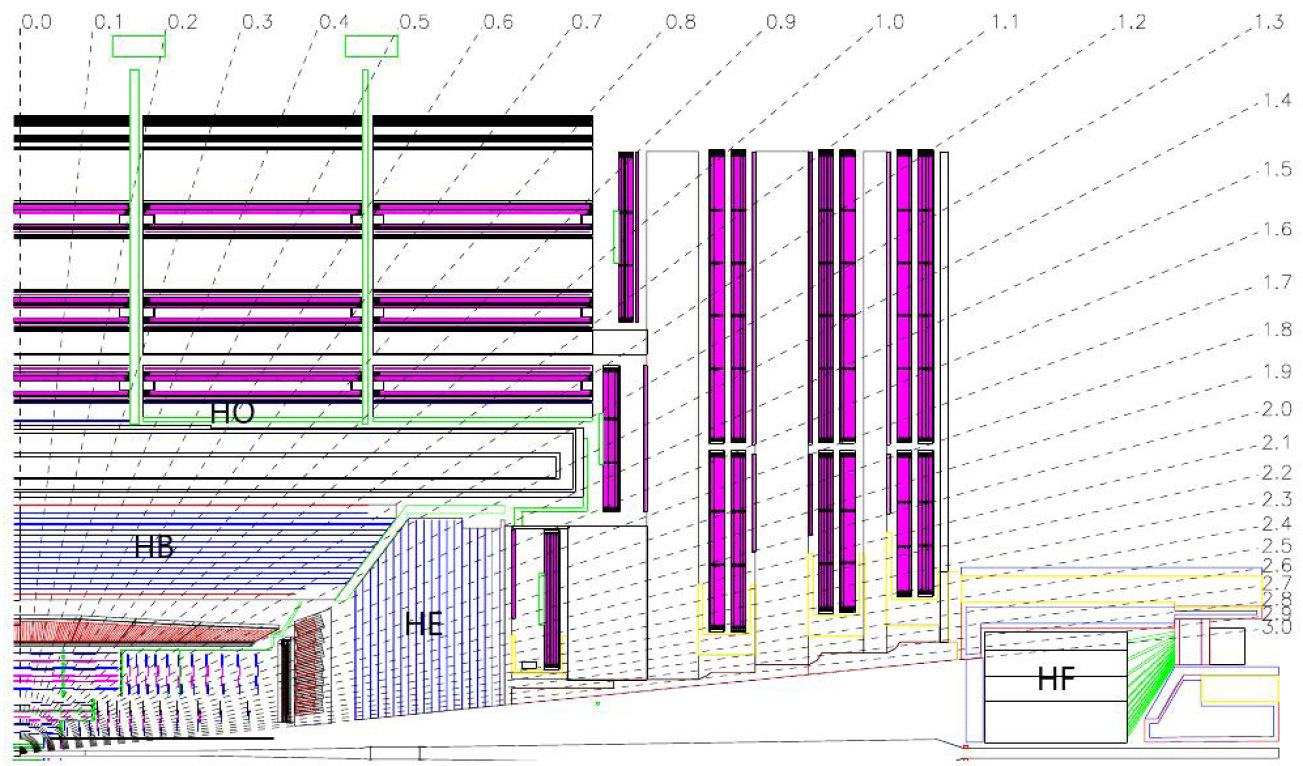
\includegraphics[width=0.8\linewidth]{figs/cms_HCAL} \end{center}
\caption{ A schematic of the \CMS \HCAL. The locations of the hadron
barrel (HB), endcap (HE), outer (HO) and forward (HF) calorimeters are
displayed \cite{Chatrchyan:2008aa}}
\label{fig:hcal} \end{figure}

The combined resolution, $\sigma_E$ of the \ECAL and \HCAL when
considered together have been measured in a test beam as
\cite{Abdullin:2008zzb}: 
\begin{equation} \label{eq:hcalres}
\left(\frac{\sigma_E}{E[\gev]}\right)^2=\left(\frac{84.7\pm1.6\%}
{\sqrt{E[\gev]}}\right)^2+(7.4\pm0.8\%)^2.  
\end{equation} 
In this equation $E$ is the energy of the incident particle. An
in-situ calibration is also performed with a UV laser and
$^{137}$Cs$/^{60}$Co sources that can be inserted into the scintillation
tiles in the \ac{HB} and \ac{HE}.

\subsection{The Muon System} 

As muons are heavier than electrons they are minimally ionising,
losing little energy via brehmsstrahlung. They therefore pass through
the \ECAL and \HCAL depositing little energy. As they are a key
component of many electroweak decays \CMS has a dedicated muon system
interleaved with the iron return yoke surrounding the solenoid. This
muon system consists of wire chambers containing ionising gas that, in
combination with the tracker, allows the measurement of muon momenta
with a greater than $1\%$ precision \cite{CMS:1997dma}.

\begin{figure}
\begin{center}
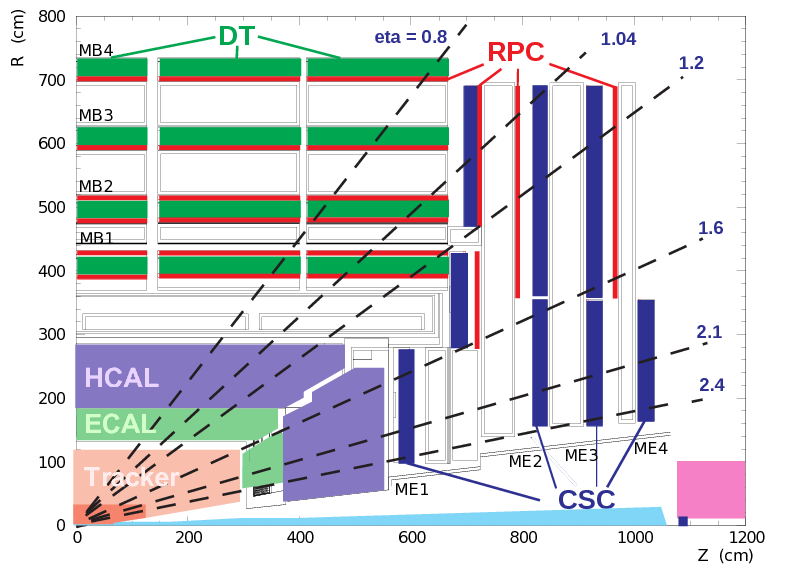
\includegraphics[width=0.8\linewidth]{figs/cms_muon} \end{center}
\caption{ A schematic of a quadrant of the \CMS muon system. The
locations of the Drift Tube (DT), Resistive Plate Chamber (RPC) and
Cathode Strip Chamber (CSC) subsystems are displayed
\cite{Kim:2012ix}.}
\label{fig:muon} \end{figure}

The layout of the muon system can be seen in Fig.~\ref{fig:muon}. It
consists of the \ac{DT}, \ac{RPC} and \ac{CSC} subsystems. They each
utilise different gaseous chamber technologies to perform measurements
of muons in different operating regions of \CMS. In the barrel region
the \ac{DT} chambers cover the range $|\eta|<1.2$. These chambers are
filled with a mixture of Ar and CO$_2$ gas. As a muon
passes through the chamber this gas is ionised. Within the chambers
are $\sim172000$ wires, each $2.4$~m long with a potential difference
applied across them. Free electrons produced in the ionisation drift
towards the anode of the wires and induce an electrical signal which
is read-out. 

Within the endcap region the \ac{CSC}s cover the range
$0.9<|\eta|<2.4$. The \ac{CSC}s are required to have a fast response
time and be radiation hard due to the higher muon and background rates
in the forward region of \CMS. They consist of chambers containing an
Ar, CO$_2$ and CF$_4$ gas mix around anode wires sandwiched by copper
cathode strips.

The \ac{RPC}s cover the range $|\eta|<2.1$ and augment the behaviour
of the \ac{DT}s and \ac{CSC}s. They consist of oppositely charged
bakelite plate electrodes separated by a 2~mm gas gap. They have a
much poorer position resolution than the other subsystems, 0.8-1.2~cm
as opposed to 40-150~$\mu$m. However they have a much better temporal
resolution of $\sim3$~ns. This allows them to be used as an
independent muon trigger that can identify the bunch crossing in which
the muon originates.

The muon systems on their own provide an energy resolution of 9-11\%
for muons with $\pT<200\gev$ and $|\eta|<2.4$. However, better
performance is obtained by combining muon chamber hits with the
tracker as described in Chapter~\ref{chap:reconstruction}. The muon
system also has excellent charge identification with a misassignment
rate of $<0.1\%$ for $\pT<100\gev$ muons.

\subsection{The Trigger and Data Acquisition System}
\label{sec:triggers} 

At 40~\mhz, the rate of collisions at the LHC is so high that it would
be too computationally expensive to reconstruct and store the
$O(1)$~MB detector read-out for every bunch crossing. As the majority
of proton collisions at the \LHC are soft scattering QCD processes,
they are not useful in the search for new physics at the electroweak
energy scale. This necessitates a multi-level trigger system that is
designed to pick out and store only ``interesting'' high
centre-of-mass physics processes
\cite{Tapper:1556311}\cite{Bayatyan:706847}. Once events have been
selected by the trigger system the chosen bunch-crossings can be
stored on tape for offline analysis. They are then centrally
reconstructed through the Grid computing infrastructure and used for
high-level physics analysis \cite{Bayatyan:838359}.

The \ac{L1T} is the first component of the two layer trigger system
and is made from custom \ac{FPGA} computational boards situated close
to the detector. This technology allows for decisions to be made with
very low latency times. As the data from a bunch crossing comes out of
\CMS it can only be stored in the read-out pipelines a total of
$3.2~\mu$s, of which $\sim2~\mu$s is required for transmitting data to
and from the detector. The \ac{L1T} must therefore make a decision on
this time scale using coarse information from the calorimeters and
muon system, with the aim to to reduce the event rate to
$\sim100$~kHz. 

A flowchart showing how the data from the different detector
subsystems passes through the \ac{L1T} can be seen in
Fig.~\ref{fig:l1t}. At the Global Trigger decision is made whether to
pass the event to the next triggering stage. The calorimeter trigger
takes calorimeter deposits at the tower level and coarsely
reconstructions physics objects. Events with high total transverse or
missing transverse energy are typically accepted.  More details of the
calorimeter trigger utilised in Run~2 are given in
Chapter~\ref{chap:trigger}. The muon trigger looks for the presence of
muons with a reasonably high energy to aid the trigger decision.

\begin{figure}
\begin{center}
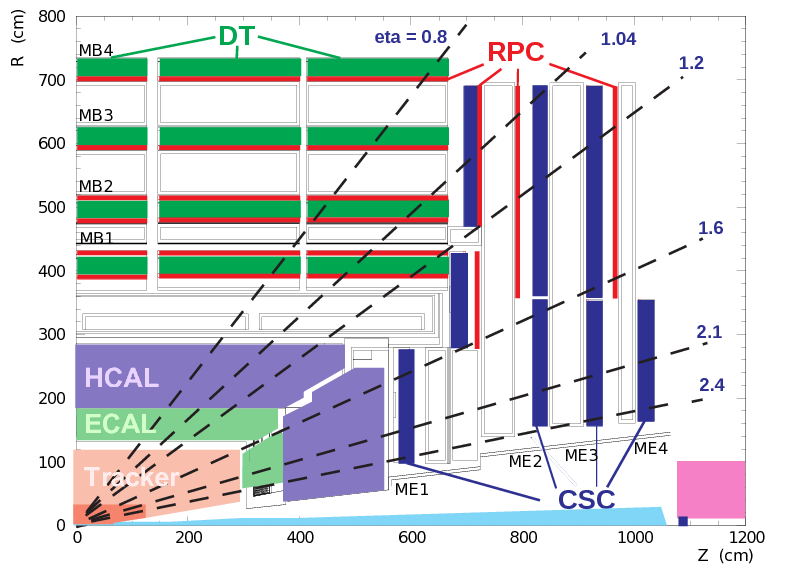
\includegraphics[width=0.8\linewidth]{figs/cms_muon} \end{center}
\caption{ Dataflow of the trigger used to collect data in Run~2 of the
\LHC \cite{Tapper:1556311}.}
\label{fig:l1t} \end{figure}

After an event has been accepted by the \ac{L1T} it is passed to the
\ac{HLT}, which uses full detector information to reconstruct the
events and reduce the data rate to $\sim1$kHz on a high-performance
computer farm \cite{Cittolin:578006}.  With reduced event rate
provided by the \ac{L1T} the \ac{HLT} has a larger latency budget, but
the algorithms used are still limited in their complexity compared to
those used for offline analysis. The \ac{HLT} tend to be tailored
towards targeting particular physics processes in a way that would not
be possible at the \ac{L1T}.
%HLT 200 ms per event

Events that are finally accepted by the \ac{HLT} are then transmitted
to the Tier-0 data centre, located at CERN, for permanent storage and
event reconstruction. This data is distributed and stored around the
world through a GRID computing infrastructure \cite{Bayatyan:838359}.
This infrastructure has a four tiered that represents the importance
and accessibility of the user at each site. From Tier-0 data are
transferred to 13 Tier-1 computing centres. These centres are then
available to Tier-2 and Tier-3 sites where offline data analysis can be
performed by different members of the \CMS collaboration around the world.
